\chapter{Introduction}
\pagenumbering{arabic}

In the past electricity production and consumption was localised to small communities. The communities often had one electricity utility company supplying the required energy. As the energy demand increased beyond single production facilities, the solution was to add more production facilities that could support in peak hours. This approach is costly, since such support facilities must be kept in a standby state, ready to deliver additional energy at a moments notice. As the electric grid expanded it began to interconnect the communities. The distribution of energy in the grid also became a challenging task. Energy must be delivered at the different consumers, at correct quantities, without overloading the grid. Furthermore must the impact errors and damages have on the grid be minimised. 

\section{Smart Grid}
As sensor technology became cheaper and more reliable the electricity utility companies started to integrate sensors in the grid. These sensors delivered information about the performance of key sections of the grid. This information was used to improve the performance of the grid. The grid grew to be more global and less local. More types of energy producing devices, such as solar power and wind turbines, got connected to it. This created a need for more control of the grid and the energy production. 

The \ab{NIST}[National Institute of Standards and Technology] is tasked with the job of creating and maintaining the standards used for the American smart-grid. The concept behind the smart-grid is to create a electrical grid that enables two way communication. Besides electricity must information about the usage also flow between the consumers and the utility companies. Usage patterns must flow to the engineers tasked with controlling the grid, and control information must flow back to the consumers or control points in the grid. This can ensure the delivery of electricity more efficiently, reliably, and securely ~\citep{RefWorks:42}. 

There are many different kind of stakeholders in today's smart-grid. In order to better understand the needs and relationships between the stakeholders have \ab{NIST} split them in to seven domains. This helps to identify the different user interest in the grid, and their needs.  

\newpage % for nice page formatting 

\begin{figure}[H]
\centering
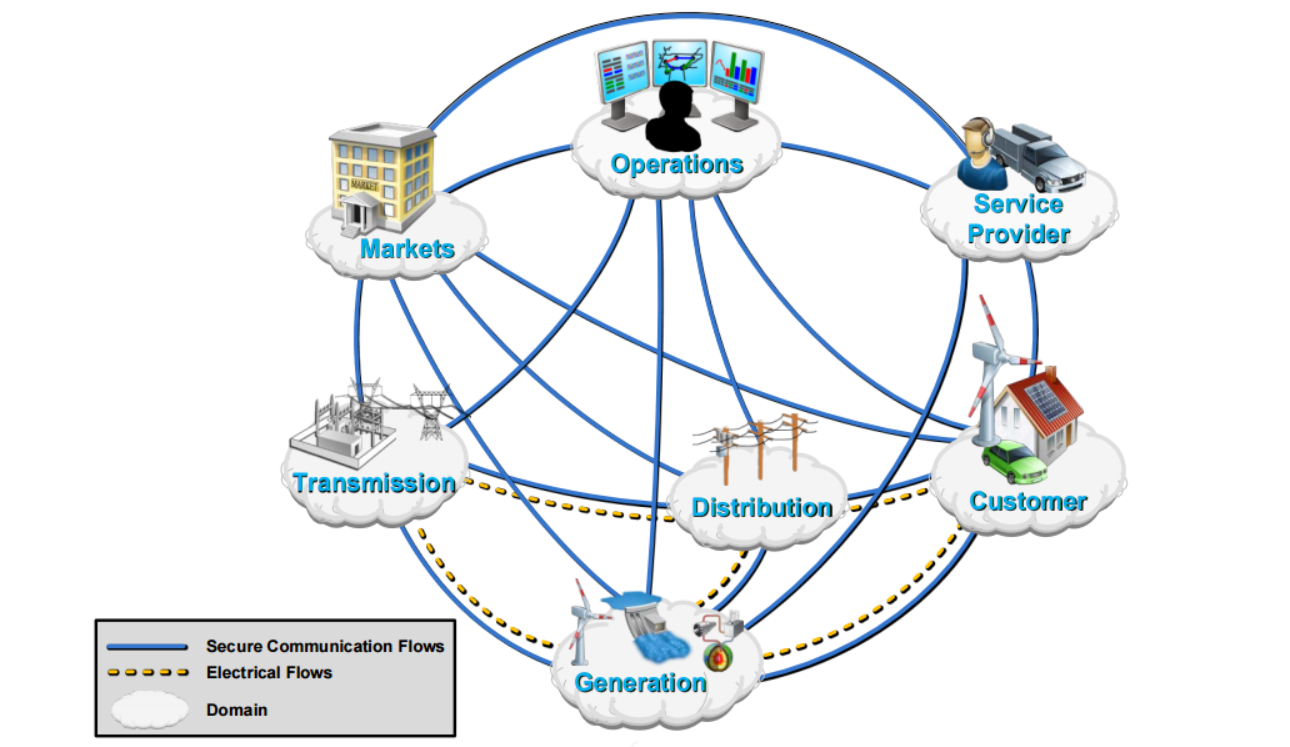
\includegraphics[width=1\textwidth]{billeder/SMARTGRID.png}
\caption{Conceptual model of smart-grid architecture. Source \citep{RefWorks:41}}
\label{fig:CMOSG}
\end{figure}
 
Figure \ref{fig:CMOSG} illustrates the seven domains. The seven domains each have a set of functions that is characteristic for the domain~\citep{RefWorks:41}.  
 
\begin{tabularx}{\linewidth}{ r X }
Generation:& Generators of electricity. This is typically coal, oil or nuclear power plants or large-scale hydro generators. This can also include energy storage facilities that stores energy for later distribution. \\\\

Transmission:& Transmission and transformers that hold the purpose of transporting the electricity over large distances. \\\\

Distribution:& The units responsible of electricity distribution to and from the customers. \\\\

Customer:& The consumers of electricity. They may also generate electricity and sell it to the grid. \\\\

Operator:& The managers of the movement and production of electricity. They are the group that ensures that the energy is efficiently delivered where it is needed. \\\\
Market:& The sale and purchase of electricity between the different instances of the grid. One utility company could purchase power from another to keep up with demand at peek hour. \\\\
Service Provider:& The organisations providing services to the utility companies or the consumer. This could be home automation or information services.  \\
\end{tabularx}

\newpage
\section{Non-Intrusive Load Monitoring}
The \df{operators} have the responsibility of controlling the flow of energy on the smart grid. This requires the knowledge of the current consumption and a prediction about the future power requirement. This prediction is generality based on statistical data collected in the grid. If the prediction of the future power requirements can be improved, it is possible to create a better and more efficient power distribution. To accomplish this is a method known as \ab{NILM} developed.

The concept of \ab{NILM} is to use the consumption information collected at household level, and use machine learning techniques to make a qualified guess on what appliances in the household is responsible for the current consumption. By using the information from the active appliances more precise estimates of future consumption can be made. 

In today's smart grid is all \df{customers} equipped with a smart-meter. The smart-meter measures the consumption of the household, and reports it back to the smart grid. This information can be used by the \df{markets} to automatically create billing information, or by the \df{operator} to regulate the power distribution. Since this information is used for distribution regulation it is send in real-time \citep{RefWorks:41}. It is this information \ab{NILM} applications hopes to use in order to create better predictions.

\ab{NILM} can also create many opportunities for the \df{service provider}. Using \ab{NILM} it is potentially possible to gesture about the usage of each appliance in a household. This can be used to better inform the resident about power saving opportunities. Studies have shown that detailed information about energy usage, makes the resident use less energy \citep{RefWorks:33}. Other business opportunities, like selling the statistical information about the usage of specific appliances might also exists.  

\section{The Problem Statement}

This report seek to investigate some of the common approaches used for \ab{NILM} today, in order to determine the capabilities of such approaches. It is assumed that such approaches is used in a modern smart grid setting. In order to answer this broad question, the following questions must be investigated. 

\begin{itemize}
\item	What quality of data can be expected from the smart-meters?\\
	
\item	How does errors and poor quality affect \ab{NILM} applications?\\
	
\item	What can we detect using  \ab{NILM} and where is the limits? \\
	
\item	Can anything be done to improve the \ab{NILM} technology?
\end{itemize}
If these question is answered it creates a strong foundation for gesturing about the the capability of \ab{NILM}. The main motivation for this study is not to improve grid load predictions, but to get a better basis for validate different \ab{NILM} related business opportunities for \df{service providers}. 

\subsection{The Data Approach}
To investigate the questions in the problem statement is the SmartHG dataset used. The SmartHG dataset is a collection of smart-meter data collected from 25 residential households in Denmark. The data is not filtered or cleaned in any way prior usage. This means that the data closely resembles what would be collected in a smart grid. Furthermore does the dataset contain information about the usage pattern of selected devices. This information can be used to compare inferred usage patterns to the actual. 
